% background.tex:

\chapter{BACKGROUND} % all caps please
\label{chap:background}
This is where the background goes. 



%%% Section
\section{Basics of Optical Imaging}
\label{chap:background:basics}

\subsection{Light-Tissue Interactions}
Biological optical imaging has the capability to detect biological structure, function, and molecular characteristics based on photon interactions with tissue~\cite{Wang2009}. The interaction of light with tissue is governed primarily by three processes: reflection, scattering, and absorption~\cite{Welch2010}.

\begin{figure}
    \begin{center}
    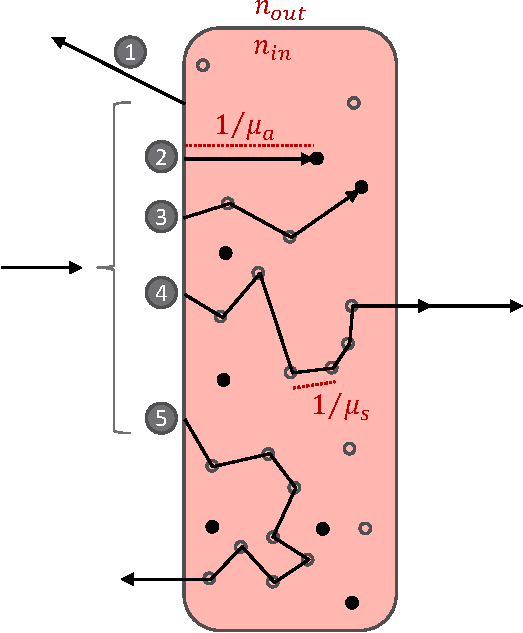
\includegraphics[width=.5\textwidth]{fig/background/lightinteraction.pdf}
    \end{center}
    \caption{} 
    \label{fig:lightinteraction}
\end{figure} 

The index of refraction, $n$, is a unitless number that describes how fast light travels through material~\cite{Wang2009}. It is used to determine how much the path of light is bent upon transitioning from one material to the next.  This is governed by Snell’s Law of Refraction~\cite{Wang2009}, $n_1 \times sin\theta_1= n_2\times sin\theta_2$, which define the angle of incidence, $\theta_1$, and angle of refraction, $\theta_2$, based on two media with indices of refraction $n_1$ and $n_2$. Thus, from Snell’s Law, we can also determine the amount of light that is reflected when reaching an interface. 

Once photons enter a turbid media, they move in all directions and may be scattered or absorbed. Absorption depends on the component concentrations of tissue~\cite{Nunez2018}. In the visible to near-infrared wavelength range, the primary absorption components include water, hemoglobin, pigment, and lipid~\cite{Du2006, Pogue2006}. The absorption coefficient, $\mu_a$ [$cm^{-1}$], is defined such that, when a photon propagates over an infinitesimal distance $ds$, the probability of absorption is $\mu_a\times ds$~\cite{Welch2010}. The absorption coefficient depends on the molar extinction coefficient of a given chromophore $\epsilon$ [$cm^{-1}\times M^{-1}$], and its Molar concentration, $c$. Thus, the absorption coefficient per wavelength is 

\begin{equation}
    \mu_a(\lambda) = log(10) \sum_{i=1}^{t}\epsilon_i(\lambda)\times c_i~\cite{Nunez2018}. 
\end{equation}
where t is the total number of absorbing components in the tissue. From this, we deduce that $1/\mu_a$ is the average path length traveled by a photon before being absorbed. 

Light entering a tissue can also undergo scattering events, events during which directionality changes occur due to biological structures within the media. In the visible to infrared wavelength range, the primary scattering components in biological tissue are protein, fat, and mitochondria~\cite{Du2006, Pogue2006}. Analogously, the scattering coefficient, $\mu_s$, is defined such that, when a photon propagates over an infinitesimal distance $ds$, the probability of scattering is $\mu_s\times ds$~\cite{Welch2010}. Additionally, we model the probability distribution of scattered photons by an angular function known as the anisotropy factor, $g$~\cite{Wang2009}. Since $g$ is based on the scattering angle, the closer to 1.0 $g$ is, the more likely the photon is to be scattered in the forward direction. To account for this anisotropy factor, we define the reduced scattering coefficient, $\mu_s^{'}$, as 
$\mu_s^{'} = \mu_s(1-g)$~\cite{Wang2009}. The average distance traveled by a photon between scattering events is $1/\mu_s$.

\subsection{Components of Optical Measurement Systems}
\subsection{Optical Phantom Fabrication}



%%% Section
\section{Imaging Modalities}
\label{chap:background:modalities}
\subsection{Pulse Oximetry}
\subsection{Functional Near-Infrared Spectroscopy}
\subsection{Diffuse Optical Tomography}
\subsection{Structured-Light Imaging}



%%% Section
\section{``-ilities'' of Near-infrared Imaging Systems}
\label{chap:background:ilities}



%%% Section
\section{Thesis Aims}
\label{chap:background:aims}


% --- EOF ---